\documentclass[parskip]{scrartcl}
\usepackage[margin=15mm]{geometry}
\usepackage{tikz}
\usetikzlibrary{fit,arrows,calc}

\begin{document}

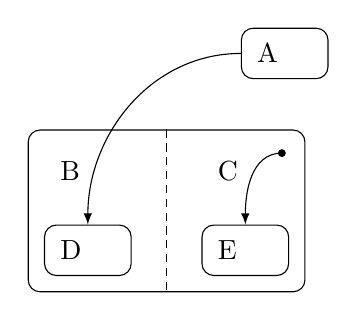
\begin{tikzpicture}
[   round/.style={rounded corners=1.5mm,minimum width=1cm,inner sep=2mm,above right,draw,align=left,text width=7mm}
]
    \node[round] (D) at (0,0) {D};
    \node[round] (E) at (2,0) {E};
    \node[above right,inner sep=2mm] (B) at (0,1) {B};
    \node[above right,inner sep=2mm] (C) at (2,1) {C};
    \node[round,fit=(B)(C)(D)(E)] (BC) {};
        \draw[densely dashed] (BC.north) -- (BC.south);
    \node[round] (A) at (2.5,2.5) {A};
    \draw[-latex] (A) to[out=180, in=90] (D);
    \draw[-latex] ($(BC.north east)+(-0.3,-0.3)$) coordinate (temp) to[out=180,in=90] (E);
        \fill (temp) circle (0.05);
\end{tikzpicture}

\end{document}
